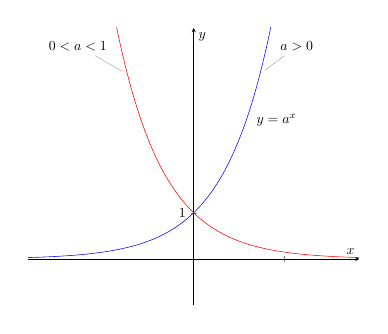
\begin{tikzpicture}[scale=0.5]
\begin{axis}[
 axis lines=middle,
 ticklabel style={fill=white},
xmin=-5.,%xmax=1.5,
ymin=-1,ymax=5,
 xlabel=$x$,ylabel=$y$,
 domain=-5:5,
 samples=30,
 smooth,
 xtick={2.7182},ytick={1},
 yticklabels={1},   xticklabels={,,},
 width=10cm]
\coordinate  (x2) at (e,1);
\coordinate  (x1) at (0,1);
\addplot[blue] {2^(x)};
\addplot[red] {(1/2)^x)};
% \fill[black] (x2) circle (1.5pt);
% \fill[black] (x1) circle (1.5pt);

%\draw[dashed] (x1)--(x2) --(e,0);
\node[] at (axis cs:2.5,{3}) {$y=a^{x}$};

\node[pin= 50:{$a>0$}] at (axis cs:2,{2^(2)}) {};
\node[pin= 130:{$0<a<1$}] at (axis cs:-2,{(1/2)^(-2)}) {};
\end{axis}
\end{tikzpicture}